% ************ Chapter 4 ************
%\renewcommand{\chaptername}{Chapter}

\chapter{Desenho \label{desenho}}
\label{cap:4}

Este capítulo incide na apresentação da forma como a framework Solid está desenvolvida até ao momento estruturada e como será estruturada a nova arquitetura proposta.

O Solid é um projeto open-source, desenvolvido principalmente por uma comunidade criada e ativamente impulsionada por Tim Berners-Lee (\emph{c.f.} \ref{estado_arte_solid}. Esta comunidade dedica os seus esforços principalmente no desenvolvimento do POD como um todo, bem como documentação e ferramentas que permitem uma mais fácil integração da solução de novas aplicações.

O pilar do Solid é a descentralização, e por descentralização entende-se redefinição da propriedade da informação e por consequência alteração de todo o paradigma subjacente à camada \emph{backend} dos sistemas actuais. No atual paradigma mais frequentemente utilizado, a arquitetura cliente servidor (\emph{c.f.} \ref{estado_arte_cliente_servidor}), a propriedade dos dados está condenada a perder-se na confiança para com a entidade de gere a camada de persistência de dados.

Numa perspetiva um pouco mais global, o que o Solid ambiciona substituir é a camada de persistência e possivelmente nas aplicações menos complexas a camada de backend também, entendo-se por complexidade a lógica de negócio que pode ou não precisar de ser assegurada em outro sistema que não a aplicação por motivos de segurança ou até mesmo performance.

As aplicações cliente (\emph{Relying Party App} conectam-se ao \emph{POD} escolhido no momento de autenticação e, através de um ontologia própria ou uma já existente, são capazes proporcionar a experiência final existente nos dias de hoje, mas garantindo que a informação está sobre alçada do seu legítimo proprietário (\emph{c.f.} figura 2.2).

Existem dois cenários possíveis de evolução do conceito Solid: (i) Manter a existência de múltiplas instâncias de Solid, e o utilizador pode escolher ao que pretende ligar-se; (ii) Existir apenas uma que pode ser entendida de forma semelhante a uma rede \emph{P2P} (\emph{c.f.} secção \ref{subsection:p2p}).

O Cenário de múltiplas instâncias corresponde ao atual e permite que possam existir globalmente diversas instâncias de POD, podendo inclusive existirem instâncias mais fechadas (por exemplo: família, empresa, etc) ou até mesmo instâncias privadas para apenas um utilizador (\emph{c.f.} figura \ref{figure_solid_multiple_instances}). Este modelo apresenta, contudo, alguns desafios de \emph{continuous delivery}, na medida em que tem de ser criados mecanismos que permitam manter todas as instâncias de POD serem atualizadas.

\begin{figure}[H]
    \begin{center}
    % Requires \usepackage{graphicx}
    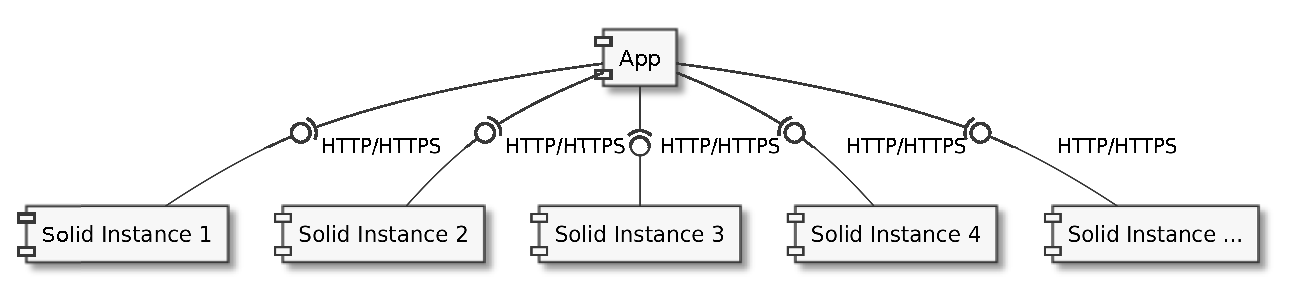
\includegraphics[width=1 \textwidth]{figures/solid_web1.eps}
    \caption{Diagrama de Componentes Solid - múltiplas instâncias}
    \label{figure_solid_multiple_instances}
    \end{center}
\end{figure}


Por outro lado, e numa perspetiva um pouco mais disruptiva, O Solid poderia evoluir para uma solução única globalmente distribuída através de uma rede de “pequenas partes” do POD que iriam comunicar entre si. Este modelo parte do principio que o Solid segue uma arquitetura orientada a micro-serviços e que estes podem executados e ligados à rede em qualquer parte do planeta e por qualquer pessoa, de forma a que iríamos assistir a uma única instância global de Solid, escalada por uma comunidade de cidadãos (\emph{c.f.} figura \ref{figure_solid_p2p_network}).
Este conceito tem obviamente sérios desafios como:
\begin{itemize}
    \item \emph{continuous delivery} - seria também um desafio neste modelo, na medida em que seria necessário garantir que todas as instâncias dos diferentes micro-serviços estão devidamente atualizados
    \item Descoberta de novas instâncias - O Solid teria de implementar um mecanismo de registo de novas instâncias para que o tráfego pudesse ser encaminhado para novas instâncias
\end{itemize}

\begin{figure}[H]
    \begin{center}
    % Requires \usepackage{graphicx}
    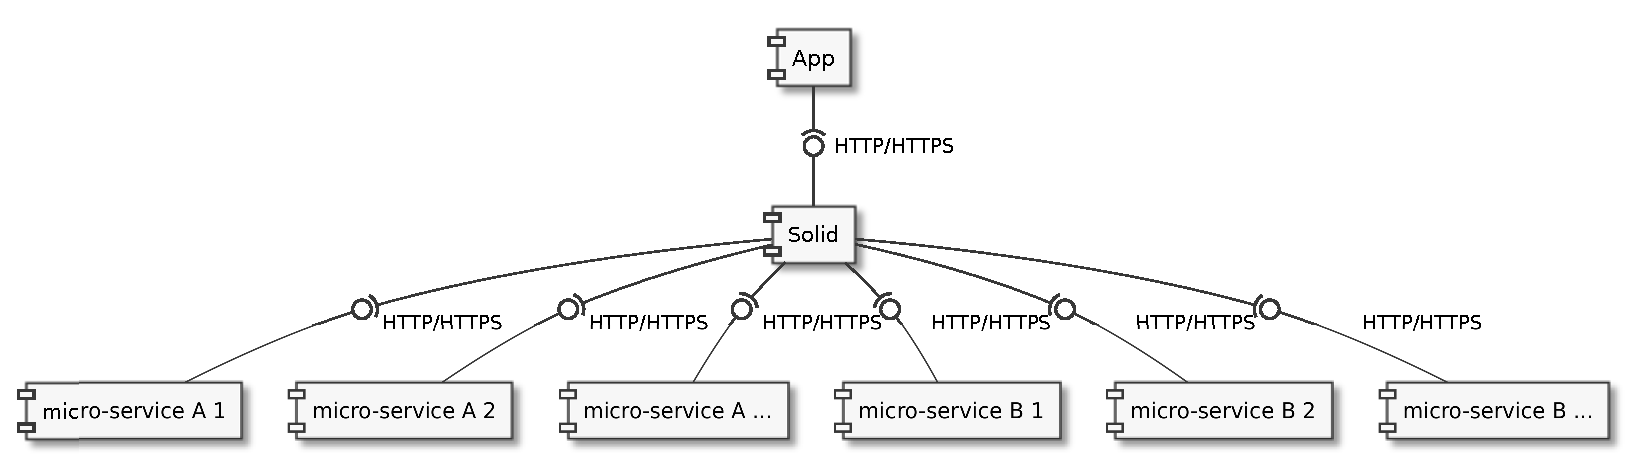
\includegraphics[width=1 \textwidth]{figures/solid_web2.eps}
    \caption{Diagrama de Componentes Solid - \emph{P2P Network}}
    \label{figure_solid_p2p_network}
    \end{center}
\end{figure}

A visão do \emph{Solid} tende a privilegiar o sentido de liberdade de escolha do utilizador, sendo possível este escolher em que instância do \emph{Solid} confia ou até mesmo criar uma instância particular ({c.f. secção \ref{estado_arte_solid}}. Neste ponto de vista, e 
de forma a cumprir a hipótese de manter a experiência para utilizador final (\emph{c.f.} secção \ref{section_hypothesis}), foi optado por seguir o modelo atual do Solid, mas com vista a migrar o Solid para uma arquitetura orientada a micro-serviços, mantendo assim as portas abertas para no futuro poder ser pensada uma evolução do modelo para uma rede distribuída pela comunidade.

Assim, nas secções que se seguem apresentam-se as alterações estruturais propostas de forma a potenciar uma migração de uma arquitetura em monólito para uma arquitetura orientada a micro-serviços.

\section{Arquitetura Proposta \label{section_arquitetura_proposta}}
Um dos problemas da arquitetura atual é a centralização de muitas camadas importantes no mesmo processo, afetando assim a sua escalabilidade, e pode consequentemente condenar o sucesso desta framework (\emph{c.f.} secção 2.1.1).

Existe, desta forma, espaço para evoluir para uma arquitetura orientada a micro-serviços, potencialmente assente na divisão por capacidades de negócio, resumindo-se estas às seguintes:
\begin{itemize}
    \item Gestão de contas - Camada responsável por garantir as operações de CRUD sobre o conceito de conta
    \item  Autenticar utilizadores - Esta autenticação consiste sobretudo em garantir que a autenticidade do utilizador e conferir acesso da aplicação cliente ao seu WebID;
    \item Autorizar acesso de utilizador a determinado recurso - Deve ser possível consultar, alterar e criar novas regras de acesso a recursos num qualquer POD existente;
    \item Aceder e efetuar operações sobre recursos - O utilizador deve conseguir (se autenticado e autorizado) efectuar operações sobre recursos.
\end{itemize}

Desta forma, a arquitetura proposta deverá ter em consideração a separação da plataforma atual em quatro possíveis componentes (cada um deles responsável por uma das capacidades de negócio identificadas):
\begin{itemize}
    \item Solid-ID - Será a camada responsável pela autenticação do utilizador, esta autenticação.
    \item Permissions - Camada responsável pela autorização.
    \item Storage - Camada responsável pelo acesso e manipulação de recursos.
    \item Accounts - Camada responsável pelas operações de CRUD sobre contas
\end{itemize}

Cada um dos diferentes componentes implementados deverá, numa perspetiva mais baixo nível, seguir uma estrutura com os seguintes módulos (\emph{c.f.} figura \ref{module_diagram}):

\begin{itemize}
    \item \emph{Controllers} - Responsáveis por gerir a lógica relativa a casos de uso. Estes podem servir de resposta a pedidos tanto por interface REST API como por via de consumo de mensagens assíncronas provenientes de um \emph{Message Broker}.
    \item \emph{Services} - Camada responsável por gerir lógica de comunicação com sistemas externos (por exemplo publicação de eventos para \emph{Message Broker} (\emph{c.f.} secção \ref{service_pattern}).
    \item \emph{Handlers} - Camada maioritariamente responsável por deter utilitários (p.e handler para erros durante execução).
    \item \emph{Models} - Módulo responsável por gerir as estruturas de dados e lógica de negócio relativa a entidades relevantes do POD.
    \end{itemize}

\begin{figure}[H]
    \begin{center}
    % Requires \usepackage{graphicx}
    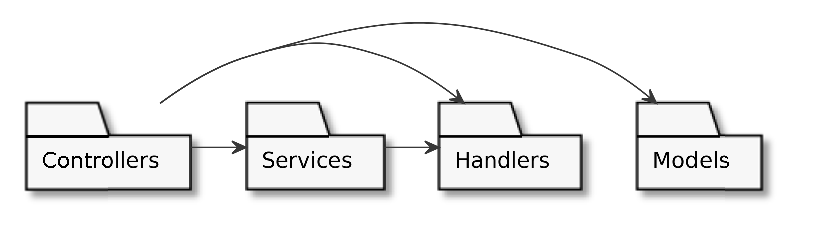
\includegraphics[width=0.6 \textwidth]{figures/module_diagram.eps}
    \caption{Diagrama de Módulos}
    \label{module_diagram}
    \end{center}
\end{figure} 


Tendo por base os componentes apresentados, são descritas nas secções seguintes duas arquiteturas baseadas em pedidos \emph{HTTP/HTTPS} com potencial para migração da plataforma Solid para micro-serviços: (i) Arquitetura não orientada a eventos  (\emph{c.f.} \ref{subsection:arquitetura_1}); (ii) Arquitetura orientada a eventos) (\emph{c.f.} \ref{subsection:arquitetura_2}).

\subsection{Arquitetura não orientada a eventos} \label{subsection:arquitetura_1}

Esta arquitetura tem subjacente a aplicação do padrão \emph{API Gateway} como o ponto de entrada para todos o micro-serviços. Este padrão (\emph{c.f.} \ref{api_gateway}) permite, desta forma, encapsular os diferentes serviços em pedidos \emph{HTTP/HTTPS}, que reencaminham o pedido para o serviço mais indicado. Esta abstração oferece vantagens como escalabilidade, segurança e monitorização (\emph{c.f.} \ref{api_gateway})

É importante denotar que todos os componentes nesta arquitetura disponibilizam apenas uma interface de aplicação REST através do protocolo \emph{HTTP}, que poderá ser seguro (HTTPS) quando a sua utilização encontra-se subjugada à utilização de um certificado válido emitido por uma entidade acreditada.

A figura \ref{component_diagram_arquitetura1} apresenta uma demonstração gráfica da interação entre os diferentes componentes nesta arquitetura.

\begin{figure}[H]
    \begin{center}
    % Requires \usepackage{graphicx}
    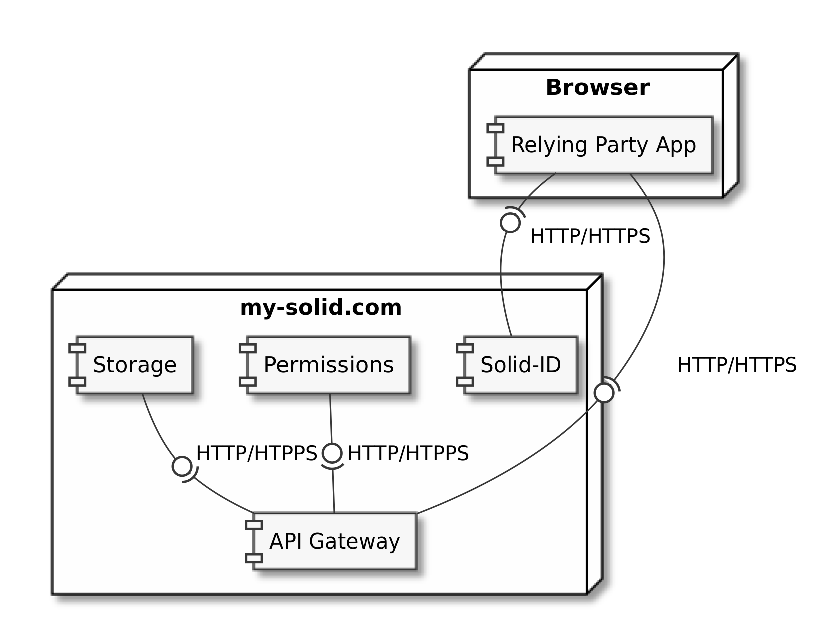
\includegraphics[width=1 \textwidth]{figures/arquitetura_1_diagrama_componentes.eps}
    \caption{Diagrama de Componentes Arquitetura 1}
    \label{component_diagram_arquitetura1}
    \end{center}
\end{figure}

\subsection{Arquitetura orientada a eventos} \label{subsection:arquitetura_2}

Esta arquitetura mantêm o conceito de API Gateway, mas introduz a adoção de mecanismos de troca de mensagens assíncrona (\emph{c.f.} em \ref{troca_mensagens_assincrona}) para a propagação de eventos lógicos para as diferentes aplicações que necessitem de os consumir (\emph{c.f.} figura \ref{component_diagram_arquitetura2}).

Na prática o que isto permite é, por exemplo, a propagação de um evento de criação de um novo utilizador. Aplicando-se, desta forma, o padrão CQRS (\emph{c.f.} secção \ref{cqrs}), contribuindo para um menor acoplamento entre as diferentes aplicações que lidam com escritas e com leituras de informação acerca dos utilizadores. Este padrão introduz indiretamente um outro: \emph{Eventual Consistency}, este por sua vez consiste na assunção de que alterações a um determinado modelo eventualmente induzirão num estado consistente no sistema como um todo. De acordo com o teorema de CAP (\emph{\emph{c.f.} secção} \ref{cap_theorem}), consistência é o parâmetro que devemos abdicar para conseguirmos escalabilidade e tolerância a falhas.

A utilização desta arquitetura permite também a adoção do padrão \emph{Event Sourcing} (\emph{c.f.} secção \ref{event_sourcing}), este consiste na persistência dos eventos de alteração de estado e permite que o estado do sistema seja obtido a qualquer momento pela "soma" das alterações de estado a que o mesmo foi sujeito.

Em termos de componentes, é possível perceber na figura \ref{component_diagram_arquitetura2} que o componente Permissions desaparece em detrimento do componente Accounts. O racional para esta decisão prende-se no facto de, na solução atual, o componente que gere as permissões baseia-se em ficheiros ACL geridos pela mesma camada que gere a restante informação para determinada conta e, desta forma, o custo-benefício de criar um novo serviço que estaria na prática a replicar o serviço que gere informação da conta pode não ser de todo justificável.

\begin{figure}[H]
    \begin{center}
    % Requires \usepackage{graphicx}
    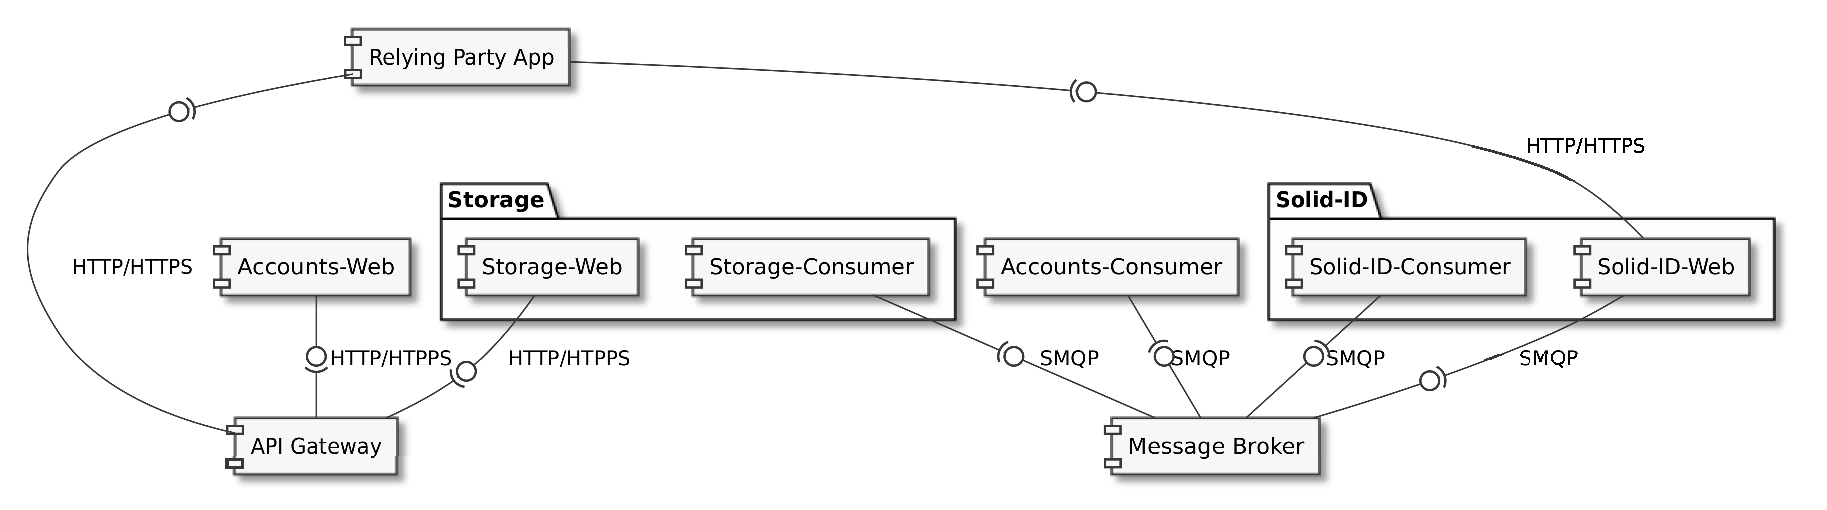
\includegraphics[width=1 \textwidth]{figures/arquitetura_2_diagrama_componentes.eps}
    \caption{Diagrama de Componentes arquitetura orientada a eventos}
    \label{component_diagram_arquitetura2}
    \end{center}
\end{figure}

\subsection{Análise comparativa \label{conclusão_arquitetura}}
Ambas as arquiteturas apresentadas compreendem uma migração para micro-serviços, sustentada numa separação em serviços baseada em capacidades de negócio.

A grande diferença entre as duas é a introdução da componente Message Broker na arquitetura baseada em pedidos HTTP e eventos, este factor adiciona complexidade, mas por outro lado, garante um maior desacoplamento entre a componente LDP e a componente ACL e garante também uma diminuição da latência na obtenção de um recurso. O ponto negativo desta abordagem é a complexidade que adiciona ao desenvolvimento e ao processo de deploy de um POD como um todo, na medida em que a sua infraestrutura será mais robusta e complexa também (\emph{c.f.} tabela \ref{table_comparacao_arquiteturas}).

\begin{table}[h]
\centering
\caption{Análise comparativa arquiteturas propostas}
\vspace{0.5cm}
\label{table_comparacao_arquiteturas}
\begin{tabular}{c|c|c|c} 
- & Arquitetura não orientada a eventos  & Arquitetura orientada a eventos \\
\hline                          
Acoplamento & Elevado & Reduzido \\
Complexidade & Reduzida & Elevada \\
Latência & Elevada & Reduzida \\
\end{tabular}
\end{table}

Assim, e tendo em conta uma decisão fundada em critérios como escalabilidade e manutenabilidade, será seguida a arquitetura orientada a eventos. Seguem-se alguns detalhes arquiteturais numa perspetiva de mais baixo nível.

\section{Casos de uso}
Nesta secção é apresentada uma vista arquitetural numa perspetiva de mais baixo nível, dando a entender de que forma os diferentes interagem no contexto dos casos de uso.

\begin{figure}[H]
    \begin{center}
    % Requires \usepackage{graphicx}
    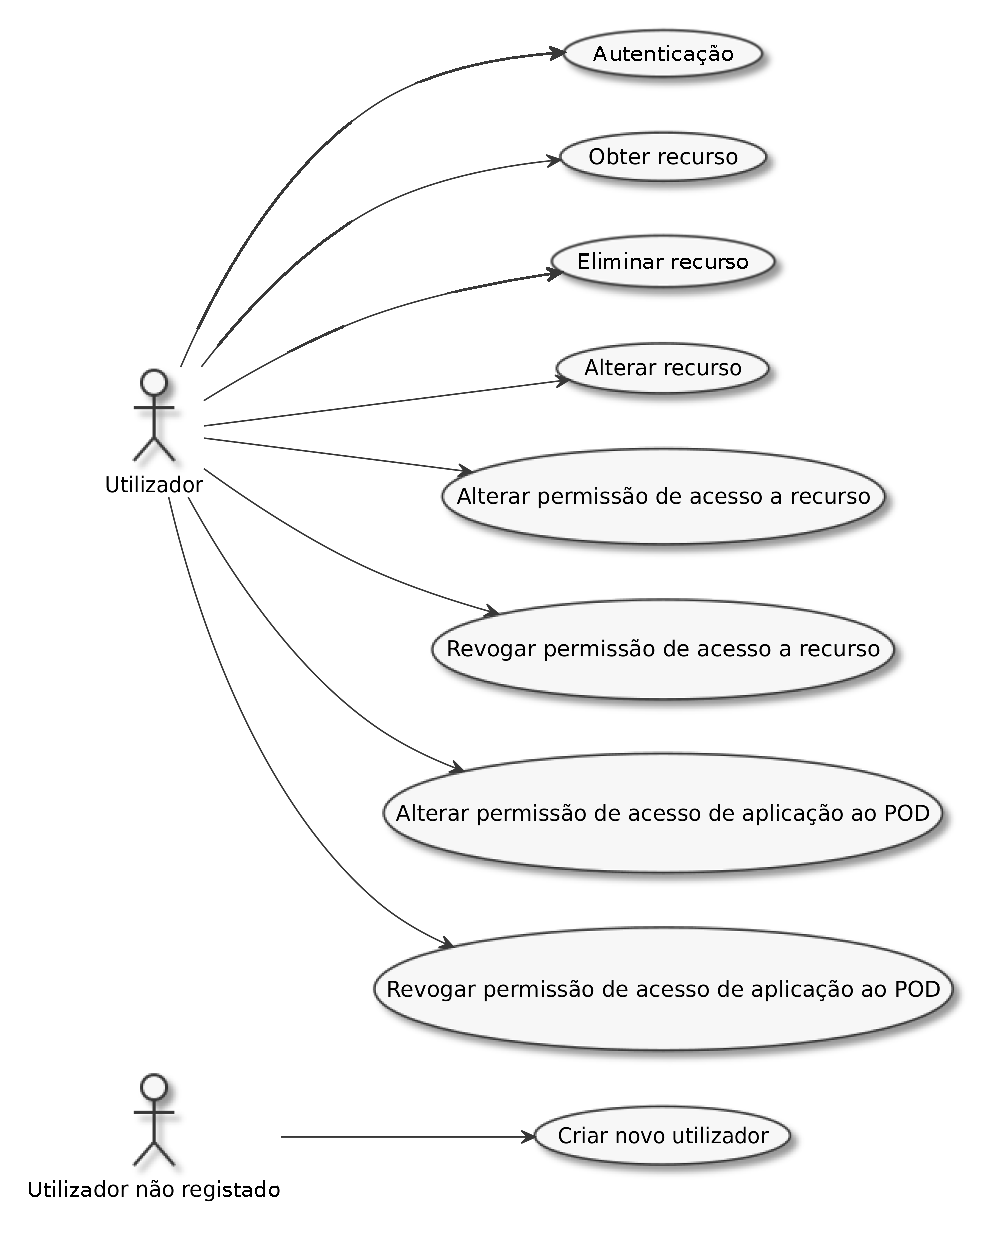
\includegraphics[width=1 \textwidth]{figures/uc_diagram.eps}
    \caption{Diagrama de casos de uso
    \emph{Solid-ID}}
    \label{uc_diagram}
    \end{center}
\end{figure}

De forma a evitar redundância de informação, está secção, de todos os casos de uso (\emph{c.f.} figura \ref{uc_diagram}), terá foco naqueles que são arquiteturalmente mais relevantes.

\subsection{Criar Novo Utilizador \label{create_user_use_case_design}}

O caso de uso de criar um novo utilizador representa uma funcionalidade arquiteturalmente relevante na medida em que implica interação entre todos os serviços constituintes do sistema Solid.

De forma a tornar mais clara a interação entre os diferentes componentes neste caso de uso, e pelo facto do diagrama de sequência ser extenso, o caso de uso é apresentado divido em nas três subsecções com os respetivos diagramas de sequência:

\subsubsection{Registo de conta}

O ponto de entrada para este caso de uso é a \emph{API Gateway} que reencaminha o pedido para o \emph{Accounts Web} através do protocolo \emph{HTTP/HTTPS}. Este, por sua vez é responsável por validar os campos preenchidos pelo utilizador segundo a lógica de negócio e no caso da informação ser válida propagá-la para \emph{Message Broker} através do protocolo \emph{AMQP} (\emph{c.f.} figura \ref{registo_conta_sd1}).

\begin{figure}[H]
    \begin{center}
    % Requires \usepackage{graphicx}
    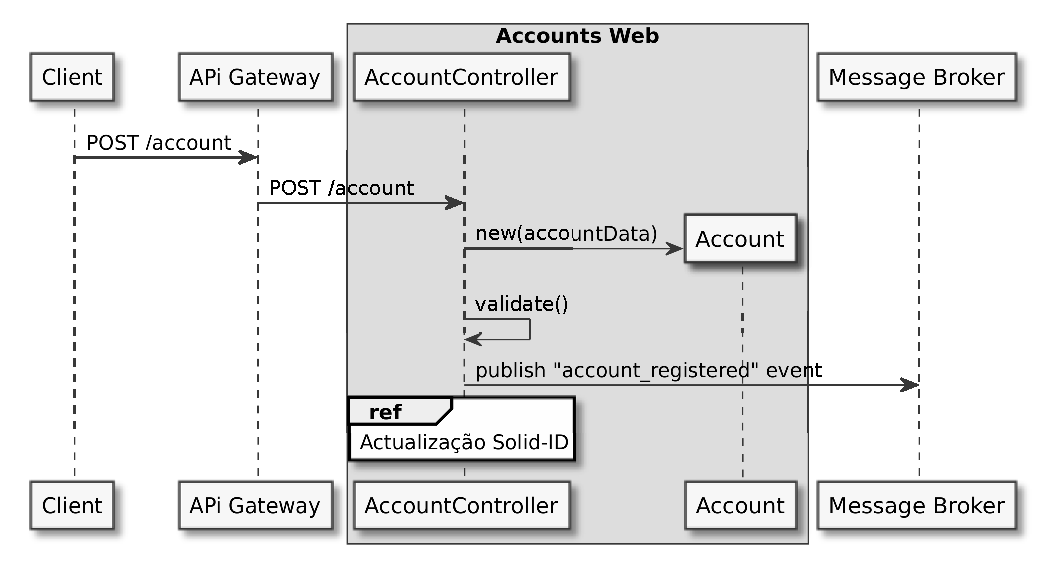
\includegraphics[width=1 \textwidth]{figures/create_account_sd_diagram_1.eps}
    \caption{Diagrama de Sequência criação novo utilizador - registo de conta}
    \label{registo_conta_sd1}
    \end{center}
\end{figure}

\subsubsection{Actualização \emph{Solid-ID}}

Assim que o evento de criação de uma nova conta chega ao \emph{Message Broker}, este encaminha-o para as \emph{queues} que estiverem configuradas para a sua \emph{routing key}. A partir desse momento, o \emph{Solid-ID Consumer} e qualquer outro consumidor  destas \emph{queues} irá processar assincronamente os eventos. O \emph{Solid-ID Consumer} é responsável por gerir a conta e todo o processo de autenticação, necessitando, desta forma, de processar este evento para que possa persistir a nova conta e propagar para os outros sistema que o conseguiu fazer com sucesso (\emph{c.f.} figura \ref{registo_conta_sd2}).

\begin{figure}[H]
    \begin{center}
    % Requires \usepackage{graphicx}
    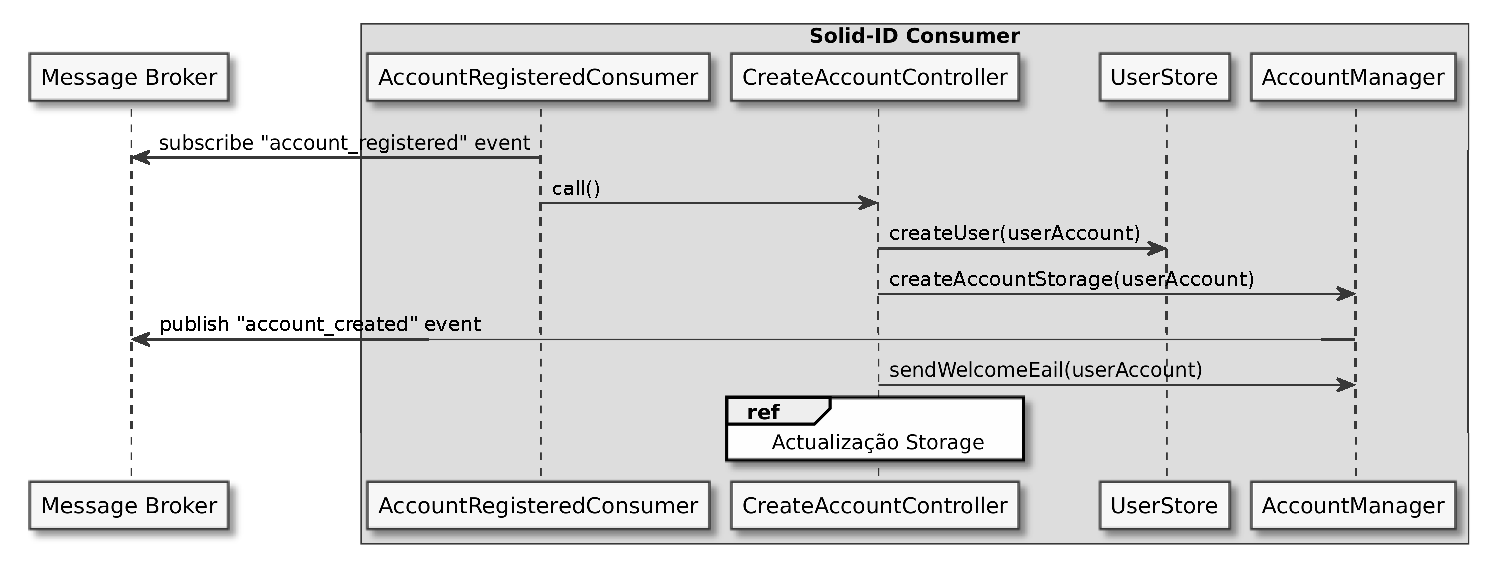
\includegraphics[width=1 \textwidth]{figures/create_account_sd_diagram_2.eps}
    \caption{Diagrama de Sequência criação novo utilizador - atualizar \emph{Solid-ID}}
    \label{registo_conta_sd2}
    \end{center}
\end{figure}

\subsubsection{Actualização \emph{Storage}}

O \emph{Storage Consumer} irá, por sua vez, processar o evento de utilizador registado com sucesso para providenciar a estrutura de ficheiros template para todas as novas contas e terminar o processo de criação de uma nova conta num POD do Solid (\emph{c.f.} figura \ref{registo_conta_sd3}).

\begin{figure}[H]
    \begin{center}
    % Requires \usepackage{graphicx}
    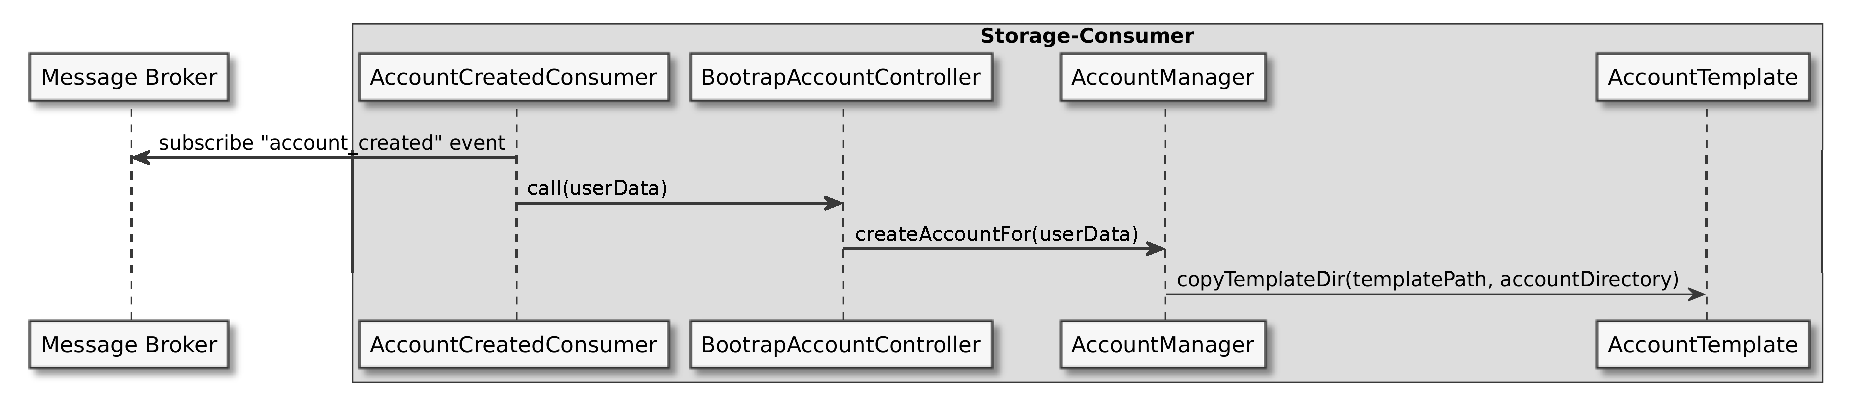
\includegraphics[width=1 \textwidth]{figures/create_account_sd_diagram_3.eps}
    \caption{Diagrama de Sequência criação novo utilizador - atualizar \emph{Storage}}
        \label{registo_conta_sd3}
    \end{center}
\end{figure}

\subsection{Autenticação utilizador \label{design_authentication}}
Nesta secção é apresentado o processo de autenticação através de uma \emph{Relying Party App}, este cenário é um dos pilares do funcionamento do Solid, na medida em que o POD terá de substituir toda a camada \emph{backend} das aplicações cliente.

Este caso de uso será também subdividido em sub-partes de forma a apresentar diagramas de sequência menos complexos e mais claros.

\subsubsection{Início autenticação}

O cenário de autenticação deverá começar com a interação numa \emph{Relying Party App}, esta por sua vez irá encaminhar para um formulário de login servido pelo \emph{Solid-ID Web}. Os dados preenchidos no formulário serão de seguida validados e o utilizador será reencaminhado para o seguinte passo se as credenciais introduzidas estiverem correctas (\emph{c.f.} figura \ref{autenticacao_sd1}).

\begin{figure}[H]
    \begin{center}
    % Requires \usepackage{graphicx}
    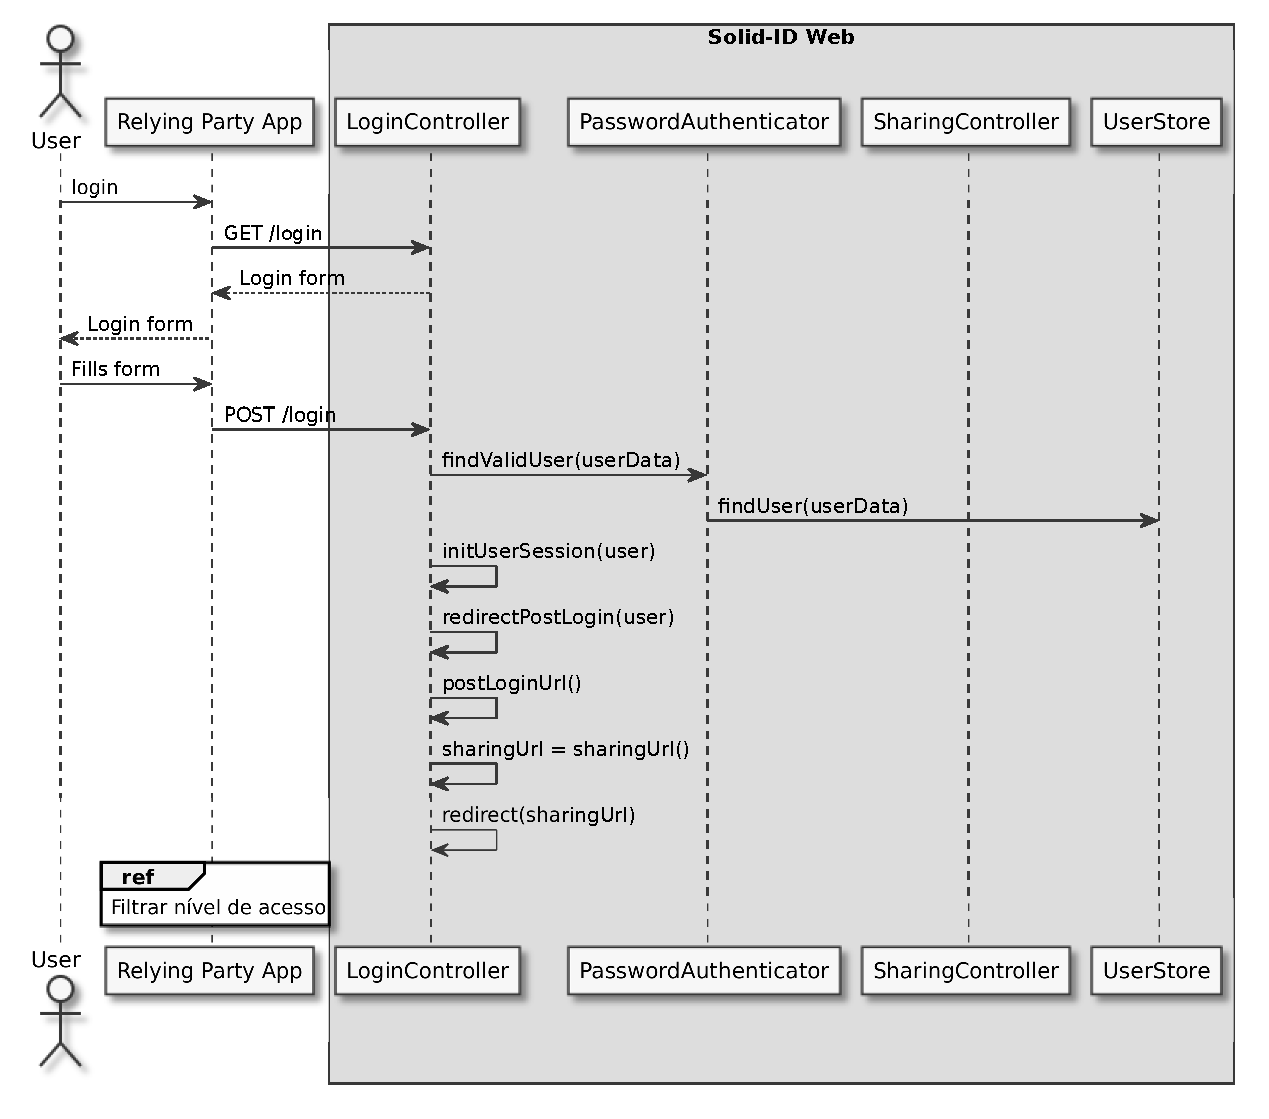
\includegraphics[width=1 \textwidth]{figures/authentication_sd_1.eps}
    \caption{Diagrama de Sequência Autenticação de utilizador - Início autenticação}
        \label{autenticacao_sd1}
    \end{center}
\end{figure}

\subsubsection{Filtrar nível de acesso}

O passo seguinte corresponde à escolha do nível de acesso da aplicação cliente aos dados no POD, esta escolha poderá ser editada pelo utilizador a qualquer altura.
Este passo só deverá ser necessário realizar uma vez, sendo que nas restantes será avançado diretamente para o passo de geração do \emph{token} de acesso (\emph{c.f.} figura \ref{autenticacao_sd2}).

\begin{figure}[H]
    \begin{center}
    % Requires \usepackage{graphicx}
    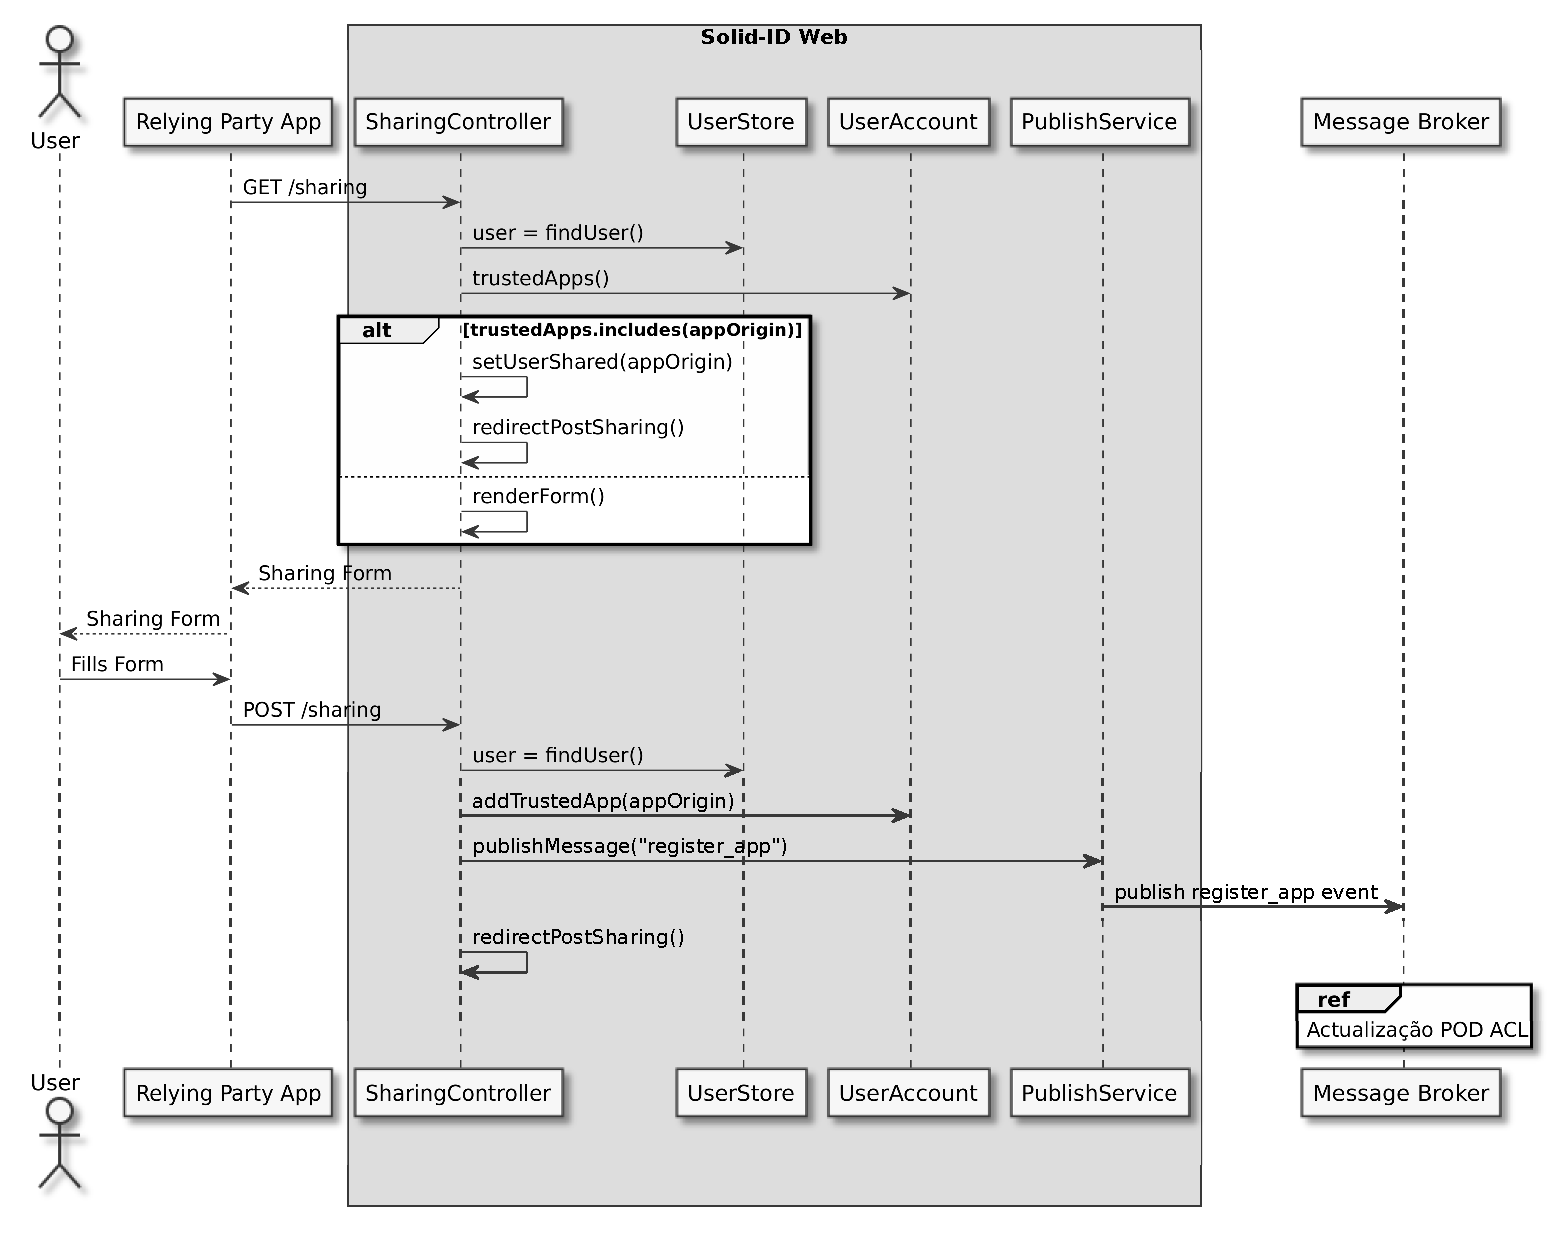
\includegraphics[width=1 \textwidth]{figures/authentication_sd_2.eps}
    \caption{Diagrama de Sequência Autenticação de utilizador - Filtrar nível de acesso}
            \label{autenticacao_sd2}
    \end{center}
\end{figure}

\subsubsection{Actulização \emph{POD ACL}}

Ainda no seguimento da escolha do nível de acesso de determinada aplicação cliente aos dados de um utilizador num POD, é necessário que essa informação seja adicionada à respetiva ACL. Para isso, o \emph{Storage Consumer} está a escutar uma \emph{queue} de eventos de registo de origens dadas como seguras e que irá adicionar aos ficheiros ACL do respetivo utilizador (\emph{c.f.} figura \ref{autenticacao_sd3}).

\begin{figure}[H]
    \begin{center}
    % Requires \usepackage{graphicx}
    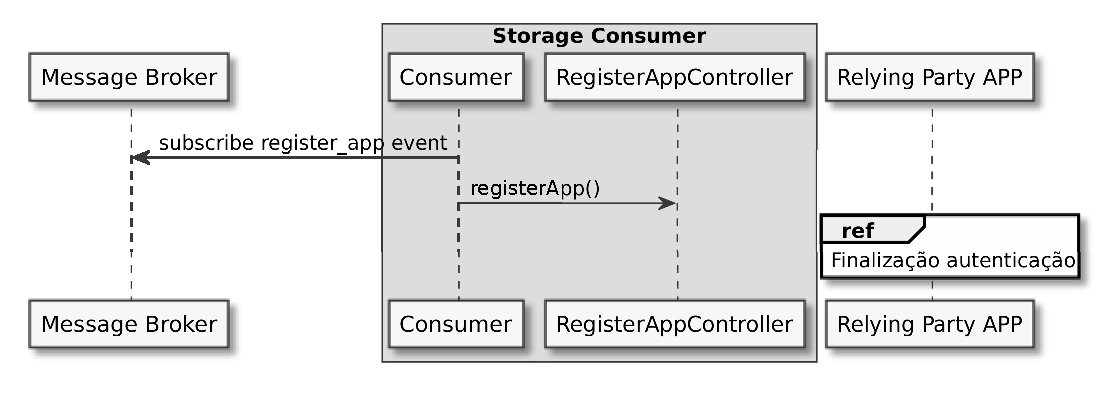
\includegraphics[width=0.8 \textwidth]{figures/authentication_sd_3.eps}
    \caption{Diagrama de Sequência Autenticação de utilizador - Actualização \emph{POD ACL}}
    \label{autenticacao_sd3}
    \end{center}
\end{figure}

\subsubsection{Finalização autenticação}

O ultimo passo do processo de autenticação corresponde a conceder o acesso propriamente dito da aplicação \emph{Relying Party App} ao \emph{POD} utilizador. Este acesso é conferido através da emissão de um \emph{token} no formato \emph{JWT} (\emph{c.f.} secção \ref{subsection:jwt}) devidamente assinado (\emph{c.f.} figura \ref{autenticacao_sd4}).

\begin{figure}[H]
    \begin{center}
    % Requires \usepackage{graphicx}
    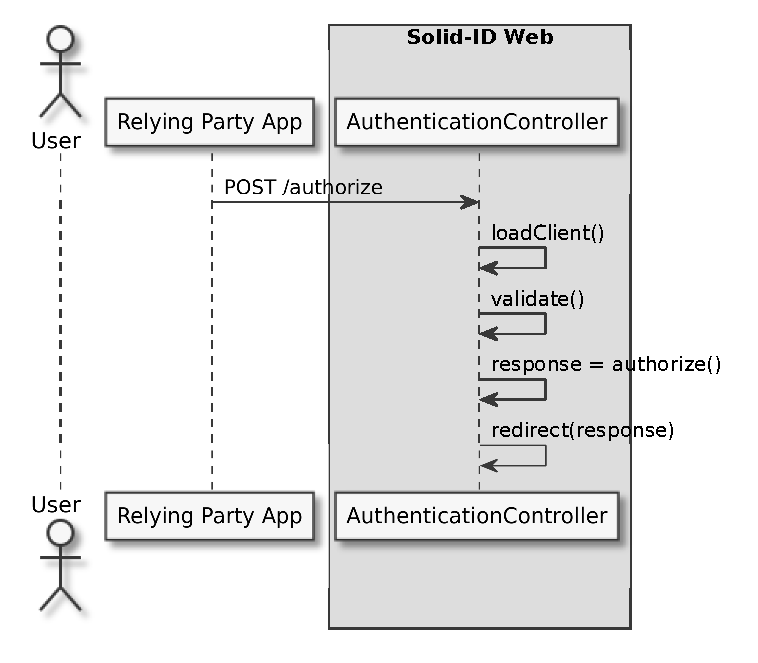
\includegraphics[width=0.6 \textwidth]{figures/authentication_sd_4.eps}
    \caption{Diagrama de Sequência Autenticação de utilizador - Finalização autenticação}
    \label{autenticacao_sd4}
    \end{center}
\end{figure}

\subsection{Obter recurso}
Este caso de uso implica aceder à unidade de armazenamento do utilizador na instância de \emph{Solid}, o POD (\emph{c.f.} secção \ref{subsection_solid_armazenamento}). 

Assim, este caso de uso inicia-se com a interação entre uma \emph{Relying Party App} e o \emph{Storage-Web}, esta interação acontece sob o protocolo \emph{http/https} e deve ser autenticada através do token de acesso fornecido do passo de autorização.
Como o token de acesso foi gerado no \emph{Solid-ID}, o componente \emph{Storage} necessita de garantir que aquele token é válido e também se pode conceder acesso ao recurso pedido.

O primeiro passo é necessário efetuar a valição do token de acesso, para tal deverá ser validada a assinatura, a data de expiração e os \emph{scopes} (\emph{c.f.} figura \ref{retrieve_resource_sd})

Após a validação do token de acesso, é necessário validar se o \emph{webID} obtido através do token tem de facto acesso ao recurso que pretende. Esta validação é realizada com recurso a uma biblioteca desenvolvida pela comunidade do Solid - \emph{ACL-Checker} - que recursivamente valida os ficheiros ACL com hierarquia sobre o recurso pretendido e analisa se o webID tem acesso e que tipo de acesso tem (\emph{c.f.} figura \ref{retrieve_resource_sd}).

A partir do momento em que os dois \emph{middlewar} (validação token e validação ACL) permitem avançar, é possível seguir para para a lógico de leitura / escrita do recurso.

\begin{figure}[H]
    \begin{center}
    % Requires \usepackage{graphicx}
    
\includegraphics[width=1 \textwidth]{figures/retrieve_resource_sd_complete.eps}
    \caption{Diagrama de Sequência Obter recurso}
            \label{retrieve_resource_sd}
    \end{center}
\end{figure}












